\begin{figure}[htbp]
  \centering
  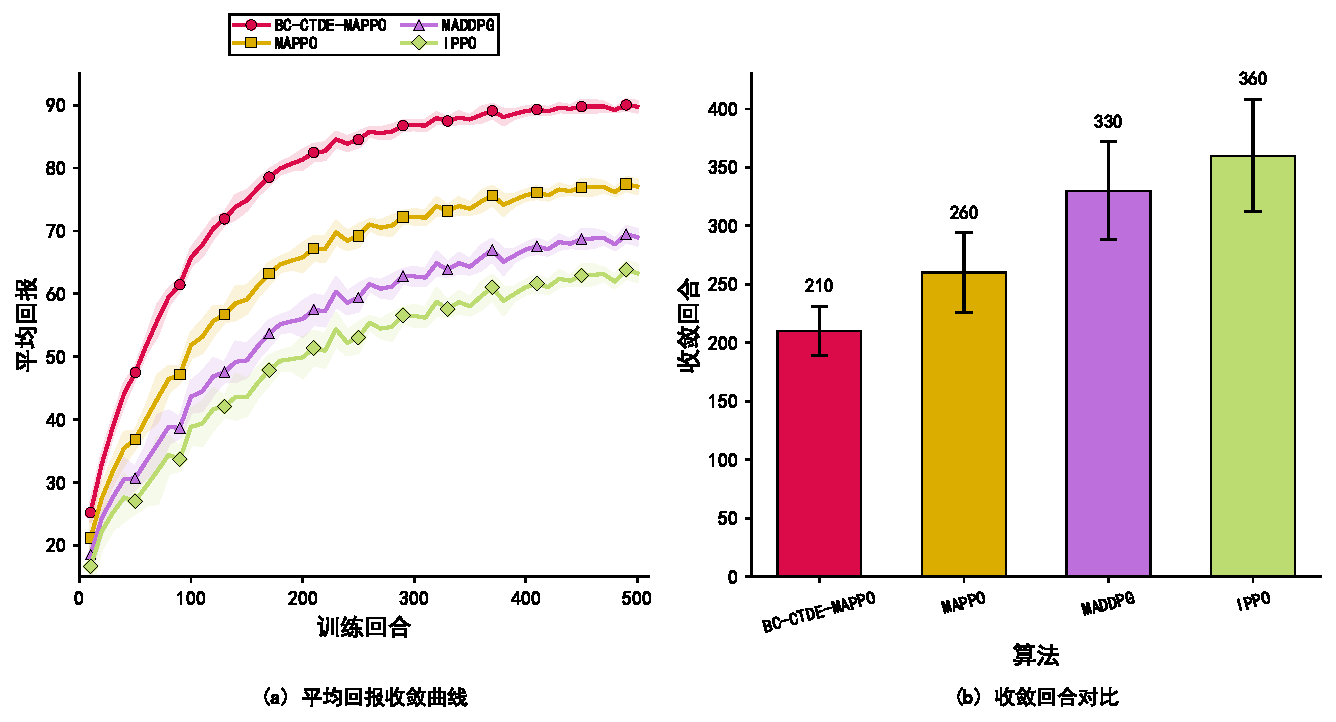
\includegraphics[width=0.98\linewidth]{chapter3_experiment_package_cn_v2/figures/fig3_6_convergence_combined.pdf}
  \caption{不同训练算法的收敛性对比}
  \label{fig:3_7}
\end{figure}

\begin{figure}[htbp]
  \centering
  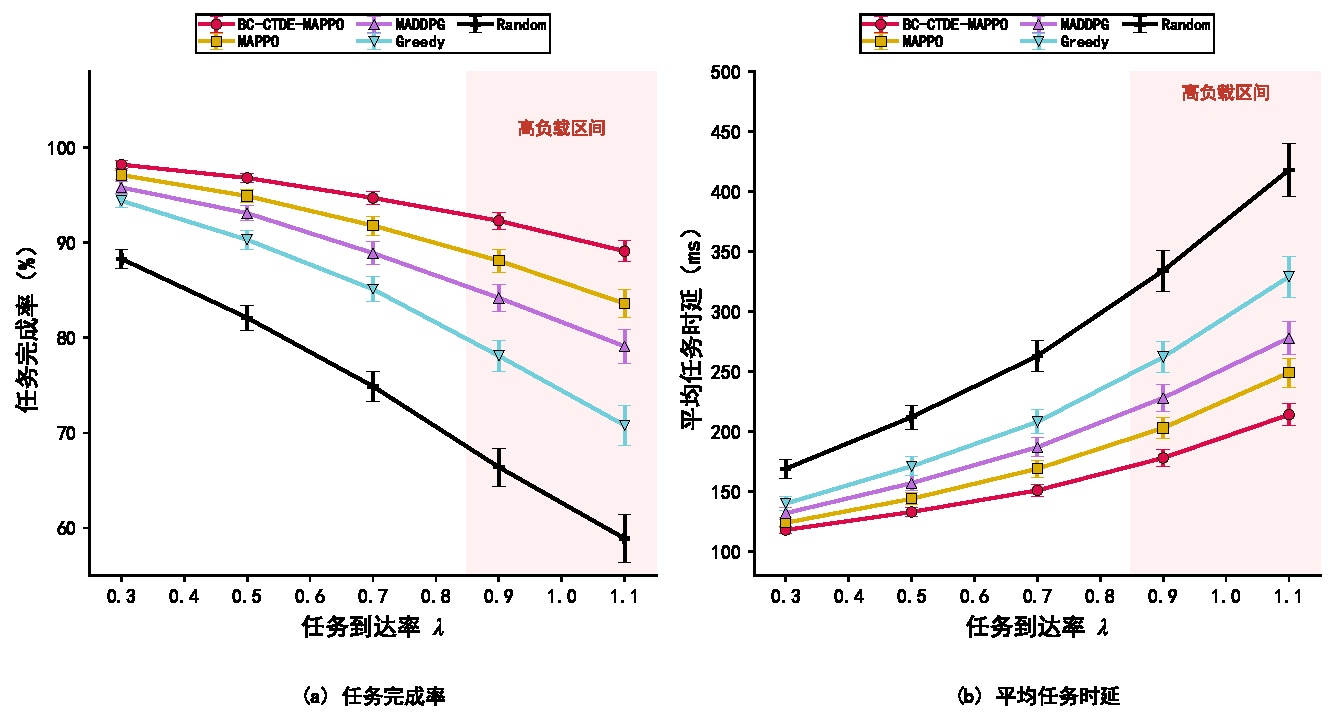
\includegraphics[width=0.98\linewidth]{chapter3_experiment_package_cn_v2/figures/fig3_7_load_performance_combined.pdf}
  \caption{不同任务到达率下的系统性能对比}
  \label{fig:3_8}
\end{figure}

\begin{figure}[htbp]
  \centering
  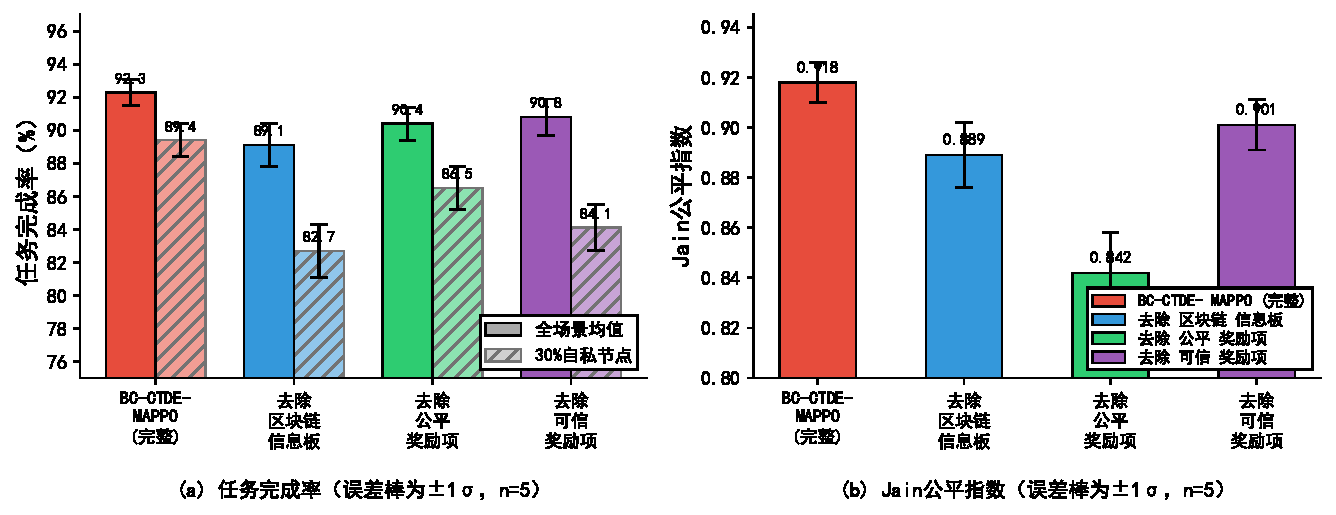
\includegraphics[width=0.98\linewidth]{chapter3_experiment_package_cn_v2/figures/fig3_9_mechanism_effect_combined.pdf}
  \caption{规模扩展与参数敏感性分析结果}
  \label{fig:3_9}
\end{figure}

\begin{figure}[htbp]
  \centering
  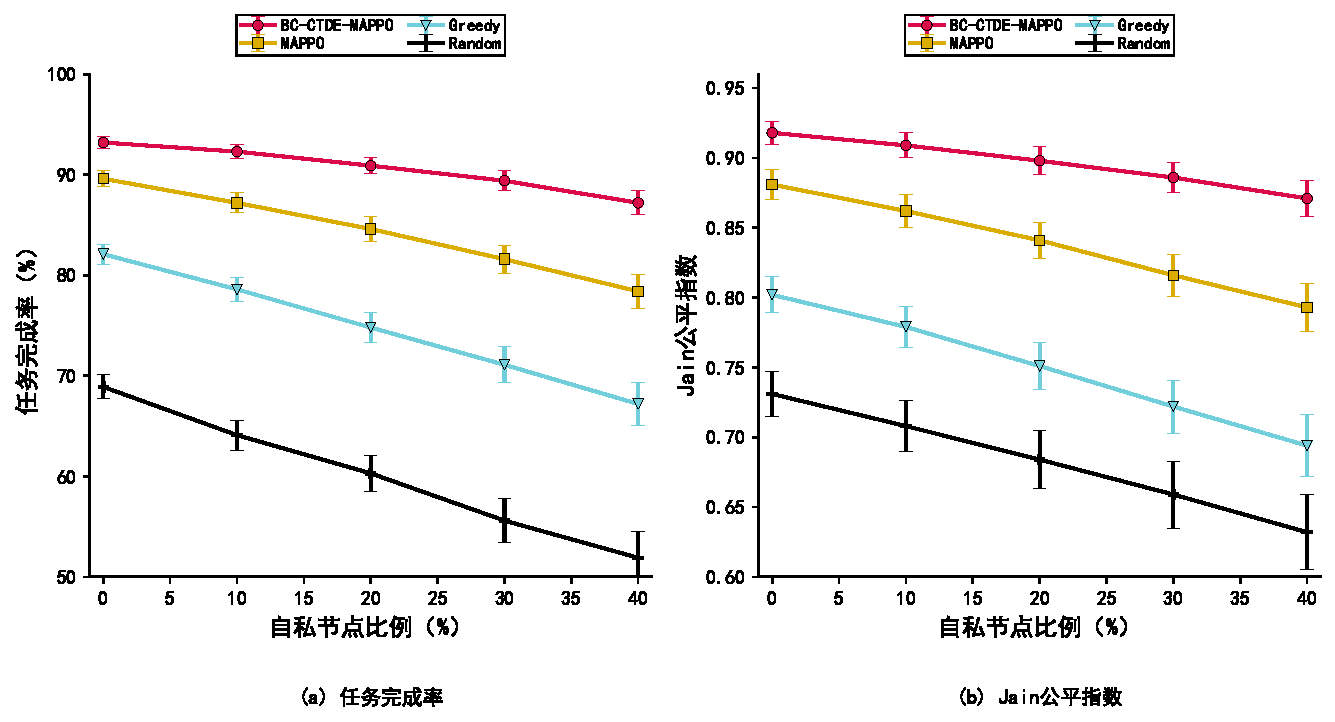
\includegraphics[width=0.98\linewidth]{chapter3_experiment_package_cn_v2/figures/fig3_8_robustness_combined.pdf}
  \caption{不同自私节点比例下的系统鲁棒性对比}
  \label{fig:3_10}
\end{figure}
